\documentclass[12pt,book]{article}
\usepackage[T1]{fontenc}
\usepackage{lmodern}
\usepackage{amssymb,amsmath}
\usepackage{ifxetex,ifluatex}
\usepackage{fixltx2e} % provides \textsubscript
% use upquote if available, for straight quotes in verbatim environments
\IfFileExists{upquote.sty}{\usepackage{upquote}}{}
\ifnum 0\ifxetex 1\fi\ifluatex 1\fi=0 % if pdftex
  \usepackage[utf8]{inputenc}
\else % if luatex or xelatex
  \ifxetex
    \usepackage{mathspec}
    \usepackage{xltxtra,xunicode}
  \else
    \usepackage{fontspec}
  \fi
  \defaultfontfeatures{Mapping=tex-text,Scale=MatchLowercase}
  \newcommand{\euro}{€}
    \setmainfont{PT Serif}
\fi
% use microtype if available
\IfFileExists{microtype.sty}{\usepackage{microtype}}{}
\usepackage[margin=1.5in]{geometry}
\usepackage{graphicx}
% Redefine \includegraphics so that, unless explicit options are
% given, the image width will not exceed the width of the page.
% Images get their normal width if they fit onto the page, but
% are scaled down if they would overflow the margins.
\makeatletter
\def\ScaleIfNeeded{%
  \ifdim\Gin@nat@width>\linewidth
    \linewidth
  \else
    \Gin@nat@width
  \fi
}
\makeatother
\let\Oldincludegraphics\includegraphics
{%
 \catcode`\@=11\relax%
 \gdef\includegraphics{\@ifnextchar[{\Oldincludegraphics}{\Oldincludegraphics[width=\ScaleIfNeeded]}}%
}%
\ifxetex
  \usepackage[setpagesize=false, % page size defined by xetex
              unicode=false, % unicode breaks when used with xetex
              xetex]{hyperref}
\else
  \usepackage[unicode=true]{hyperref}
\fi
\hypersetup{breaklinks=true,
            bookmarks=true,
            pdfauthor={Justin Murphy},
            pdftitle={The Pacification of the World: Notes on the Politics of Information and Communication},
            colorlinks=true,
            citecolor=red,
            urlcolor=red,
            linkcolor=red,
            pdfborder={0 0 0}}
\urlstyle{same}  % don't use monospace font for urls
\setlength{\parindent}{0pt}
\setlength{\parskip}{6pt plus 2pt minus 1pt}
\setlength{\emergencystretch}{3em}  % prevent overfull lines
\setcounter{secnumdepth}{0}

%%% Change title format to be more compact
\usepackage{titling}
\setlength{\droptitle}{-2em}
  \title{The Pacification of the World: Notes on the Politics of Information and
Communication}
  \pretitle{\vspace{\droptitle}\centering\huge}
  \posttitle{\par}
  \author{Justin Murphy}
  \preauthor{\centering\large\emph}
  \postauthor{\par}
  \date{}
  \predate{}\postdate{}


\usepackage{setspace}
\onehalfspacing


\begin{document}

\maketitle


\begin{abstract} 
Though a great deal has been written on diverse political implications of information technology, and models of political economy now routinely include information considerations, there does not yet exist a general political theory of information technology. This manuscript outlines a series of theoretical and empirical notes to this end. In the most general terms, I argue that advancements in information technology tend to empower challengers of a status quo in the short-run but, through multiple causal pathways, ultimately strengthen the political stability of a status quo in the long-run. My argument explains why nearly all dominant political categories have come to ring hollow, diverse types of social trust have been depleted, and system-level political contention has been pacified and erased from memory in the wealthy liberal world since the 1970s.
\end{abstract}

{
\hypersetup{linkcolor=black}
\setcounter{tocdepth}{2}
\tableofcontents
}
\section{Part 1: General Theoretical
Reflections}\label{part-1-general-theoretical-reflections}

\subsection{Fragments}\label{fragments}

In the 1960s there was massive and widespread \emph{system-level}
political contention in many countries around the world.\footnote{By
  \emph{system-level political contention} I simply mean public
  political speech and behavior which challenged the distribution of
  power and resources at the level of institutions. By institution I
  only have in mind a basic sociological definition such as any shared
  understandings, backed by force or not, which effectively structure
  the behavior of individual agents. In this sense I understand a
  political or economic \emph{system} to be simply a set of
  institutions.}

Beginning in the 1970s, there was then an equally widespread decrease in
system-level political contention which was, in long-term historical
perspective, remarkably rapid and comprehensive. Crucially, this
pacification of system-level contention occurred at the behavioral
\emph{and} ideational level. That is, politically contentious behavior
at the system-level (for instance, general strikes, assassinations,
riots, guerrilla warfare, revolutions, etc.) saw a precipitous decrease,
but at the same time, the content and intensity of public culture became
strikingly less contentious with respect to institutions. This is simply
another way to summarize a large set of well-known observations, many of
which will be explored in the pages to come, including the rise of mass
consumerism (in commerce), the decline of unions and rise of
business-speak (in the workplace), the decline of artistic
counterculture and the rise of commercialized and individualized
replacements such as ``DIY" culture, individualised forms of political
radicalism (second wave to third wave feminism, social anarchism to
lifestyle anarchism). What all of these movements have in common is that
they represent behavioral and ideational shifts away from collective
opposition to institutions and toward individual-level struggle within
institutions which are taken for granted.

To document and explain this surprisingly under-reported empirical
puzzle, I will make a series of arguments that focus on the nature of
information in politics. These arguments lead to the following argument,
which will of course require some effort to adequately unpack. I will
argue that the information revolution led to an uneven but worldwide
shift in ethical and behavioral orientations. By increasing the payoffs
to instrumental rationality (exploitative human action based on
maximizing efficiency of means) relative to substantial rationality
(honest/dialectical/cooperative action driven by ultimate goals),
individuals and organizations with exploitative ethics were
significantly more empowered by the information revolution than those
with cooperative ethics. In a process of incentivized learning, there
was a massive defection from substantial rationality (and system-level
political contention against institutions and for human liberation from
the domination of institutions) to instrumental rationality
(individual-level adjustment to institutions).

There's a crucial distinction, emphasized in particular by the Frankfurt
School, between instrumental and substantive rationality. Broadly,
instrumental rationality is that type of rationality concerned with
calculating means to ends and substantive rationality is that type of
rationality concerned with understanding the whole (means and ends).
Instrumental rationality is concerned with strategy, calculating how to
get \emph{anywhere} the most efficiently, whereas substantive
rationality is concerned with trying to figure out where one should go
in general.

The distinction emerges over and over again in politics.

\begin{itemize}
\item
  the personal integrity of anarchism vs the instrumentalism of marxism
\item
  ethos and elan vs a separate realm of strategy (that is, even
  activists notion of ``goal, strategy, tactics'' begs the key questions
  of how to live and therefore simply skips precisely to the battlefield
  in which it has already been crushed)
\end{itemize}

Because the public sphere has been so completely subordinated to
instrumentalism---the only speech which is even sensible is that which
meets some minimal threshold of self-interest, because nothing else is
credible---the most preliminary efforts to establish a genuinely kind
and loving contact with another human being are basically
impossible---let alone build radical ties or a social movement! This
extraordinary change, and undeniable \emph{decay} in communications has
never before been fully identified, let alone explained. This also
explains why today all currently existing social movements are
completely unable to build anything which can even pretends to challenge
the dominant institutions.

Instrumental communication is a means to some end which is not
communicated in the message. That which seeks to make the receiver do
something at the cost of some transparency (treats them as a means to an
end; the first goal is to achieve something for the speaker's
interests).

non-instrumental communication is an end in itself which the
communicator says for no reason other than whatever satisfactions are
brought by saying it. Or importantly, if there is a larger end to
speaking it, this is included in the message. Non-instrumental
communication therefore treats the receiver as an end in themself,
because the only instrumental value the communication can bring is
through the autonomous action of the receiver after learning
transparently the contents of the message.

They are perhaps never fully one or the other, but the argument here
does not require absolute purity. It is enough to mark out objectively
the consistent markers of the one and other. There has always been a
conflict between instrumental communication and non-instrumental (let's
call it sincere) communication. Typically, historically, instrumental
communication is the communication of the relatively powerful and
sincere communication is the communication of the powerless;
additionally, instrumental communication is the communication of the
powerful as well as the powerless in spaces and times relatively
characterized by power struggle (in a job interview, for instance, where
someone is obviously and consciously involved in a competition to win
the means to sustain one's life), whereas sincere communication is the
communication of all people in spaces and times relatively insulated
from power struggles (with loved ones, for instance). While these types
of communication have always co-existed, for most of human history they
have been in equilibrium. Before the printing press, ruling elites in
any particular society did not have an advantage in exercising
instrumental communication over their subjects. They had symbolic
machinery no doubt, but the subjects had what since time immemorial has
been the most powerful communicative structure: being socially embeded
among others in a concretely shared, if rarely equal, co-production of
life. Indeed, to this day, it is known very well that one's attitudes
and behaviors are most crucially shaped by one's ``primary group,''
precisely the individuals by whom one is surrounded on a day-to-day
basis. Thus, the instrumental communications of the powerful have always
been held in check by structures within which sincere communication
prevailed. The lies of kings might have been obeyed because the balance
of power forced subjects to accept them, but the history of human
society shows amply that wherever domination prevails there also
prevails the wisdom of the relatively weak who, sometimes laughing and
sometimes crying and sometimes in silent gestures, always ultimately are
the only bulwark which refutes the self-interested communications of the
dominant.

However, since the industrial revolution, profound changes have occurred
in this communicative balance of power.

In periods where the ability for a particular source to reach many
people increases, there is always a sudden appearance of revolutionary
political communication and revolutionary political upheaval. But after
this opening, that which was so powerful for the forces of sincerity is
exploited for instrumental purposes. While anyone can pursue their
instrumental purposes after a sudden increase in the ability to reach
people, almost by definition the most powerful will be able to spread
their instrumental communications more widely than the less powerful.

(always quicker to the punch precisely because that which is sincere and
organic is always waiting to explode, whereas that which strategically
manipulates can only respond, hence we call this ``reactionary''.)

I propose a thesis regarding how this has been caused in history. There
has always been a conflict between the instrumental communication which
and non-instrumental communication. \textbf{Whenever the ability for one
location to contact multiple other locations increases, this empowers
both sincere and instrumental communications in the short-run. But in
the long-run, instrumentalism extends its reach more than sincerity.}
There is one main problem. In short, the ability to use this
communication is conditioned by the distribution of power, so that only
those with the resources to use the technology can use it for either
sincere or instrumental communications. Some fraction will use it for
sincere and another will use it for instrumental, but the degree to
which it used for either will be determined largely by how much those
with power to use it are invested in the status quo institutions. If the
fraction of people to use communication technology benefit from the
status quo, even sincere use of it will only be liberating for that
fraction of the people, as they will be intersted in communicative
liberation but not at the cost of their privileges. This is the example
of liberals in the Dewey camp during WW1. In a more already-equal
society, increases in communication

\paragraph{1820-1875 first upturn of
globalization}\label{first-upturn-of-globalization}

telegraph, newspapers, amateur radio first international, revolutionary
upsurges, Fanelli goes to Spain

\paragraph{1875-1914 down turn of
globalization}\label{down-turn-of-globalization}

recuperations within the left, state-corporate control of radio, second
international, anarchist terrorism as last gasping breathe. watering
down of ``democracy'' as republicanism in 1875. ww1 as corporate-state
lockdown. bolshevism.

\paragraph{1949-1975 upturn of second globalization (without
people)}\label{upturn-of-second-globalization-without-people}

trade, mass media internationally, anti-colonial war, information
revolution about 1950.

\paragraph{1975-1991 downturn of second globalization (without
people)}\label{downturn-of-second-globalization-without-people}

neoliberalism, mass media solidification, trade and investment
integration, collapse of soviet instrumentalism, mass evactuation of
left sincerity in favor of left instrumentalism within capitalism.

\paragraph{1994-2011 upturn of the networked
world}\label{upturn-of-the-networked-world}

zapatistas up to arab spring and occupy, flowerings of sincerity.

\paragraph{2011-Today downturn of the networked world, the pacified
world}\label{today-downturn-of-the-networked-world-the-pacified-world}

capitalism as mainstream ideology of most people rich and poor, left and
right. the main ideological cleavage is between ruthless instrumentalism
and humane instrumentalism, but the pole of sincere, substantive ethical
and political truth opposed to instrumentalism has been vanquished from
most of the globe. the internet.

\subsubsection{How Instrumental Rationality Favors the Right and
Inhibits the
Left}\label{how-instrumental-rationality-favors-the-right-and-inhibits-the-left}

The problem of most left political thought and practice since time
immemorial is that, because they are generated precisely by exploitative
institutional arrangements, the only left messages which receive
recognition within such cultures are those which respond to the material
needs of the exploited. This is perfectly understandable, because the
material needs which sustain life are both ethically and practically
prior to any possible social movement on other grounds. This is why
normatively lofty or aesthetically-driven currents of leftist political
thought and practice are always mocked in every period: when some people
are starving, rhetorical flights of any sort do \emph{seem} to reflect
mistaken priorities. Thus it is that mature and decent leftists always
tend to discipline the younger more ``idealistic'' leftists into calming
their normative and rhetorical passions in favor of the hard work of
getting material gains for the most exploited people. While this is
perfectly understandable and quite natural to sympathize with, there is
an extraordinary problem with this tendency. Specifically, it grants to
the exploitative institutional arrangements their most crucial ethical
and epistemological assumption: instrumental rationality. It is
necessary for the exploited to practice the instrumental rationality
required for survival, but the problem is that because of this need, the
left capitulates \emph{in general} to instrumental rationality as the
proper analytical orientation to social and political struggle. Anything
which opposes instrumental rationality is, to the committed and
\emph{rational} leftist, a prodigal self-indulgence of an immature and
``privileged'' soul uneducated in the history of the Practical Left.

Nevermind that the history of the Practical Left is a history of
betrayal, capitulation, and ultimately, complete failure---given that
domination and exploitation not only continue to exist but in the
institutions of global capitalism institutionalized more powerfully than
ever before in the history of humanity.

\subsection{skill-biased technological
change}\label{skill-biased-technological-change}

One reason is that improvements in information are a type of
``skill-biased technological change'' in which the relatively more
educated see their power increase more than the less educated, but this
is not unique to information technology. The crucial and unique
implication is that, at least within market societies, advancements in
information-processing bias all social communication toward status quo
assumptions. Despite the widespread belief that new information
technologies enhance democracy and cooperation, I argue that in the
long-run, improvements in information-processing increase the
profitability of instrumental or exploitative communication relative to
cooperative or goal-driven communication. This is because those most
invested in the status quo will use advancements in
information-processing to advance themselves within the status quo
rather than change the status quo as such; this forces those who would
otherwise seek to change the status quo to speak and behave in agreement
with the assumptions of the status quo in order to survive. While such a
dynamic emerges for many types of technological innovation, only
improvements in information-processing have such unique and far-reaching
negative externalities on the public sphere because, while skill-biased
technological change in industry might lead some workers to earn more in
the factor, skill-biased change in information-processing leads some
individuals to earn more from everyone in their life in general. For
these reasons, the information revolution sparked a process in which all
communication around the world is increasingly only instrumental
communication, and the substantial communication required for
individuals and communities to challenge elites is increasingly
evacuated. This accounts for why, today, nearly all dominant political
categories ring hollow, diverse types of social trust are depleted, and
militant political resistance to the status quo has been pacified and
erased from memory in the short span of about thirty years.

\subsubsection{The conservatism of everyday
speech}\label{the-conservatism-of-everyday-speech}

(Rephrase because this is in pamphlet.)

Everyday words do not communicate, they are much better understood
oppositely: they are blockages of communication, evolved to divide,
channel, distort, and otherwise institutionalize the human community to
increase utility of the most powerful groups. It is one of the largest
and most powerful set of mechanisms for maintaining capitalism because
they are the million little signposts which at every moment point to
people which roads pay. At every fork in our road, at those specific
moments when we do have the resources to choose good or evil, words
always send us toward capitalism because words (logos) at best are
merely true (a car which doesn't come with an engine, let alone fuel).
Logic and reason are motion-neutral, ``disinterested'' objective
analysis cannot tell anyone what to value, as only subjective desire and
commitment can propel and direct a person's projects --- but in a
dynamic system \emph{defined by} the instrumental exploitation of
humans, then disinterested logos and ratio is exploitation. Strong
logical reasoning is always paid because good thinking always strays and
is always at risk of overthrowing the status quo. Words provide the
service of absorbing a society's cognitive capacities into channels
which prevent volatile shifts of group movement. And we are simply paid
to use those words which absorb or mystify or deflect human desire into
a desire for capitalism. We earn nothing if we use words which fail to
channel human desire into exploitation, and finally we are punished to
the degree our words challenge or inconvenience powerful actors.

\subsubsection{Economic premium to computational
thinking}\label{economic-premium-to-computational-thinking}

A huge problem with the information age is that because computational
skills are rewarded disproportionately, and the top calculator minds
quickly become privileged by the status quo, what comes to be counted
and calculated tends to be motivated by a blithe confidence and
satisfaction with the institutions of the status quo.

\subsubsection{Principled Contentious
Action}\label{principled-contentious-action}

We might call ``principled contentious action'' anti-institutional or
anti-systemic political behaviors grounded in truth claims this is what
has been pacified there are still some contentious uprisings and there
are still people making truth claims but these have been separated, and
that is the crucial mystification which defines our world. but zola was
also very strategic, how is that different than today? being strategic
in a principled campaign is different than today, which is generating
principles to serve strategic ends. in the former, ends are sincere but
the means are strategic. in the latter, means are sincere but the ends
are dishonest. zola took radical strategic action in pursuit of forcing
truth and justice, even if he did it strategically; non-profit
organizations use claims of truth and justice as a vehicle for
strategically promoting certain groups.

\subsubsection{Understanding the nature of commercial
bias}\label{understanding-the-nature-of-commercial-bias}

mass media have not programmed people to think or act in a certain way,
they simply disconnect popular \emph{resistance} from the reality of
political affairs

the mechanism through which they do this is simply giving people what
they want to hear and see. this is acknowledged by every media scholar
to be a fundamental fact of commercial media. but it's effect is to
create ``noise'' in the democratic mechanism whereby people positively
or negatively to political affairs. Because by definition people are
receiving what they want, the bias is not left or right but rather media
are biased in favor of system-level dynamics and against within-system
dynamics. This is how we can account for the perplexity that people
often think the media is TOO critical of politicians AND that it is not
critical enough.

but it's not just noise in the sense of random noise, it is by
definition reinforcing of what they already think and feel and believe.
this sounds like it might push radicals to be more radical and
conservatives to be more conservative but this is wrong. why? because of
a fundamental assymetry between left and right, which spatial models of
politics fail to account for.

summarize the spatial model. that's useful but quite poor in a key
respect.

the right is whatever political reality is. the left is the desire to
change the status quo to bring it more in line with justice. the right
is that the status quo is justice and the change they promote is to stop
those efforts.

thus, commercial media is inherently conservative. it has the effect of
reinforcing the status quo (the right) by giving people what they
already want, rather than connecting them to whatever might be wrong
with the world, thus pacifying the crucial inputs which historically
lead people into contention with dominant powers.

what exactly has been pacified? principled contentious action. there's
still contention because there's plenty of ways to be contentious
roughly in support of the status quo. what has been foreclosed is
resistance to the status quo based on ethical or spiritual commitments.
instrumental contentious action persists, because instrumental
contentious action is the dominant mode of life sanctioned and
encouraged by the status quo.

principled contentious action is not left or right. like marxists didn't
support dreyfus, and some bourgeois political moderates did. if there is
anyone who embodies it, it's the radical public intellectual of theory
and action.

\subsubsection{Keynes and the False Promise of Taming
Capitalism}\label{keynes-and-the-false-promise-of-taming-capitalism}

\begin{enumerate}
\def\labelenumi{\arabic{enumi}.}
\item
  Someday we will look back on the notion of markets as we today look
  back on the witch trials: as a mass-delusional catastrophe in the
  ethical history of the world.
\item
  It is not that markets don't exist, it is not even that markets don't
  work. The problem is precisely that they do work.
\item
  The problem with Keynseianism is that by arguing that markets don't
  always work, it maintained the assumption of instrumentalism.
\item
  Keynes severely interrupted the revolutionary tendency, not because he
  was wrong, but because he was right.
\item
  Leftists in general pacify themselves with moralism. It prefers to
  feel ethically and morally righteous over getting things right.
\item
  Getting it ``right'' requires us to admit that conservatism is
  ``right,'' it is not \emph{false}.
\item
  To be radical is to choose to get it wrong with respect to the status
  quo, because one sees the status quo as wrong.
\item
  Today our ``left'' is so oriented toward being true within the status
  quo that it is unable to be anything other than the status quo.
\item
  It has been forced to seek truth within the status quo because mass
  media significantly increased the gains to being true within the
  status quo relative to saying the status quo is wrong. Globalization
  has multiplied this effect for the same reason. And since the late
  1960s there's been a remarkable though essentially invisible ethical
  re-orientation toward consistency with exploitation.
\end{enumerate}

\subsection{Sketch of a general model (a distributive theory of
information
technology)}\label{sketch-of-a-general-model-a-distributive-theory-of-information-technology}

As informational efficiency rises, all social actors are empowered to
the degree their work involves manipulating information. This is why the
1950s and 1960s saw many relative improvements in the lives of so many
actors in the United States: executives of many stripes and perhaps most
interestingly in the advertising and marketing sectors (``Mad Men''),
consumers (the golden age of suburban idyll), and social reformers (60s
radicalism and minority movements) were all empowered to some degree by
the new informational powers.

But it also increases the short-term payoffs of manipulation relative to
cooperation. Basically, increased information powers have the structure
of a prisoner's dilemma. Consider a new information power which can be
used to either cooperate or manipulate, a radio for instance. If two
people agree to use the radio to increase their cooperation by telling
each other truths, they each face what we might call a vulnerability
cost but gain what we might call a solidarity value. However, if one of
them promises to tell the truth but actually lies about their own type,
they pay zero vulnerability cost while still gaining the other person's
loyalty. The dominant strategy is to present a false type, and thus it
is that in the long-run every advancement in information power actually
incentivizes manipulative falsity.

The period from 1947 to 1973 was essentially the first stage of learning
process, where various strategies for maneuvering in the digital world
are experimented with. Cooperators cooperated more powerfully (the
extraordinary potency of late 1960s radicalism), but manipulators also
manipulated more powerfully, and the beginning of the 1970s was just the
point at which the remaining cooperators defected in the face of a
seemingly unstoppable reality of manipulation as destiny. Indeed, the
late 60's in particular is a last gasping breathe against
instrumentality, and the 1970s marks its defeat by instrumental reason
and begins a global ethical race to the bottom, where the left is sucked
into a huge global vacuum, pulled either into the orbit of neoliberalism
or mystified postures of protest merely bought and sold on the market.
Hence all the radicals who gave up the radical struggle and opted for
status quo media manipulation (consider the remarkable example of the
Latin American revolutionary who laid down arms and went to work for a
global PR firm, I have to find the citation for this\ldots{}) or
revolutionary media manipulation (even left-wing terrorism is only a
manipulative propaganda of the deed).

The real casualty on both sides of the political divide was the truth
and the radicalism and solidarity unique to human honesty.

One vector of this contention is played out in the rise of marketing
understood broadly as the manipulation of human beings for earning
profit, including the evolution of the marketing individual. This
becomes scientific and massive for the first time ever, it's
scientificity is evident not only in elite practices such as
quantitative marketing research but even in the most horrid and peculiar
subcultures such as that of male ``pick-up artists'' who try to develop
a vulgar science of manipulating women.

Another vector of this contention is played out in the organization of
production processes. The rationalization of economic production as well
as political (bureucratic or legal or military or ``policy'')
production.

But these vectors are really only relatively specific instances of
engineering ``operations,'' a generic term in computer, engineering, and
management sciences for any process of manipulating inputs to generate
certain outputs.

\subsubsection{The Connection Between Media and
Globalisation}\label{the-connection-between-media-and-globalisation}

The crucial connection of media and globalisation is this: as media
increased the reach of any particular message (beginning within the
nation state and then beyond it), this radically increased the payoffs
to speaking consistently with the status quo. When the ability to speak
globally occurred, this amplified it. At the same time, the same thing
that made this communication possible (the digital revolution) also
amplified the political and economic premium to education/skills.

When the amount of people any one person could reach was very small, it
was worth it to resist status quo temptations and speak against the
status quo. First of all because capitulating to the status quo did not
get you much, and second because others who suffered under the status
quo were unlikely to have much emotional investment in it (or at least
there was no reason to believe they did, a crucial point regarding the
logic of mass communications).

But as the potential reach of a status quo platform increased, this
incentivized leftists to drop the radical discourse and trade it in for
a hugely widespread but overall small positive effect rather than fight
for system change. First because the payoff of a moderate message
increased (you reach more people) but second because of the increasing
belief that everyone else supports supports the status quo (because
everyone else is getting pro-status quo messages).

\section{Part 2: Historical Outline}\label{part-2-historical-outline}

\subsection{Phase 1: The Rise of Mass Media,
1917-1968}\label{phase-1-the-rise-of-mass-media-1917-1968}

The notion of ``democracy'' as an internationally recognized and
supposedly desirable feature of national political systems is relatively
new. It is only around the time of World War I that ``democracy'' makes
its debut as a recognizable ideology of national governments. More
specifically, it was ony a relatively small group of Allied elites who
launched this term into mass political consciousness in order to create
public support for war against Germany.

The graphs below use data from Google Books to show that World War I is
associated with a noticeable spike of public interest in ``democracy''
and that up until recently ``democracy'' co-varied with ``propaganda.''
The data is from \href{https://books.google.com/ngrams}{Google Ngrams},
which basically counts the occurrence of phrases from millions of books
in multiple languages.

\begin{figure}[htbp]
\centering
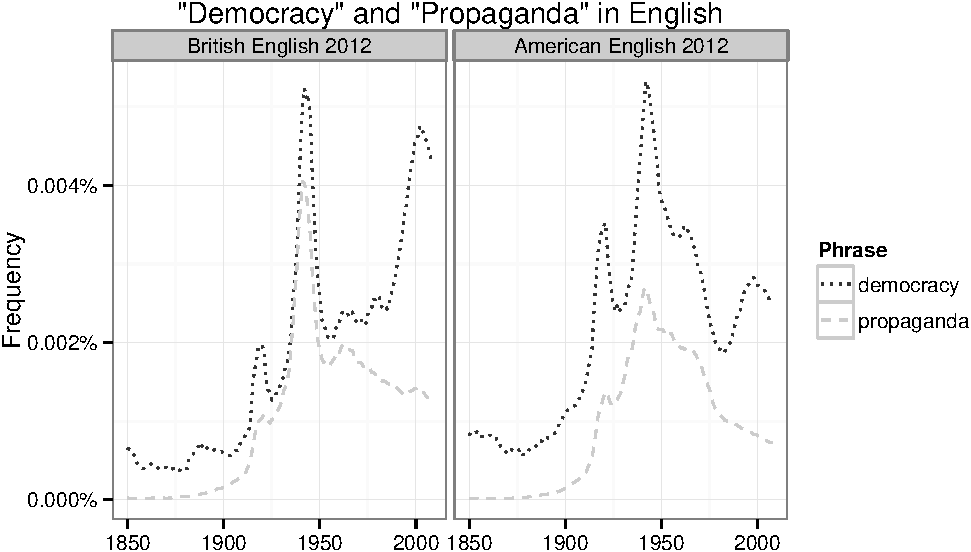
\includegraphics{pacification_of_the_world_files/figure-latex/unnamed-chunk-2.pdf}
\caption{plot of chunk unnamed-chunk-2}
\end{figure}

Strikingly, although ``propaganda'' and ``democracy'' covary throughout
most of this period, a break occurs in American and British English
after World War II (and especially beginning in the 1980s) in which the
appearance of ``propaganda'' declines while ``democracy'' increases. The
word ``media'' however, rises throughout this period. We might
hypothesize that ``media'' effectively becomes a more politically
palatable term for the same essential social machinery previously known
as propaganda. Needless to say, while the data here are consistent with
this hypothesis, they are very far from demonstrating anything in
particular.

\begin{figure}[htbp]
\centering
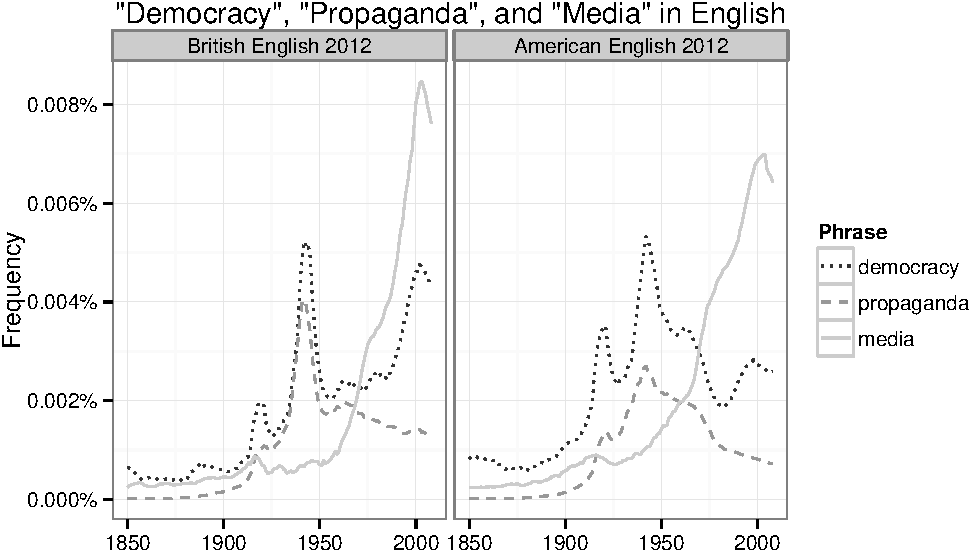
\includegraphics{pacification_of_the_world_files/figure-latex/unnamed-chunk-3.pdf}
\caption{plot of chunk unnamed-chunk-3}
\end{figure}

We find a similar pattern in French but with notable differences.

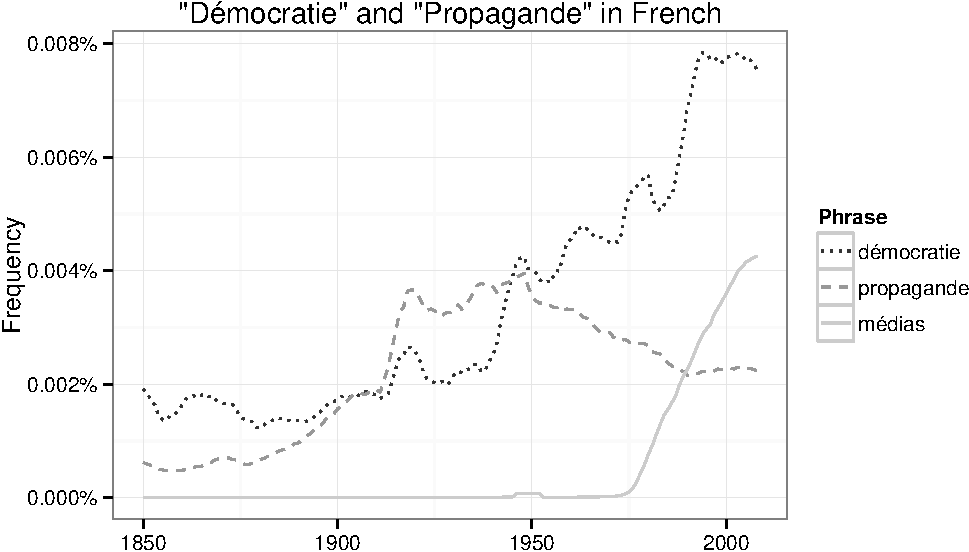
\includegraphics{pacification_of_the_world_files/figure-latex/unnamed-chunk-4.pdf}
\#\#\# The Creation of Public Opinion

It is also around this time that the notion of ``Public Opinion'' gains
serious currency, as in the writings of someone such as Walter Lippmann.
Specifically, its emergence appears to have relied on the extraordinary
success of American and British propaganda during World War I. It only
became possible to speak of something called ``public opinion''
\emph{after} national elites succeeded in using radio and newspapers to
hammer millions of diverse hearts and minds into a mass public desire
for war against Germany.

It is possible to get the impression today that only in the past few
decades has the desire of the masses ever received close, systematic
attention from government officials, as if only recently popular
sovereignty has become scientific. But the desire of the masses has
always been critical in politics, and has always been given close
attention. Autocrats have always had to ensure that they not deviate too
far from the desire of the masses, because that's when they get deposed.
Public desire has always been important, and has always been studied by
the ruling class, as a problem. There is very little evidence for the
uncritical assumptions of contemporary political scientists that the
study of public opinion is for the purpose of helping government
officials better execute the will of the people. Here, interpretation of
modern polling data using the language of political radicalism is far
more consistent with the historical evidence than ``common sense''
language: the study of public opinion today is for the purpose of
ensuring that the masses never get too angry.

Whenever public opinion falls too low, something can always be done as a
response; something to appease the masses and restore their faith in the
system. The scientific study of public opinion, however, transforms the
desire of the masses into the demands of the masses. And this is why it
is one of the most marvelous counterrevolutionary devices ever evolved.

Beginnings:

\begin{itemize}
\item
  Ironically, it was the French Minister of Finance in the years just
  before the French Revolution who first pointed out the importance of
  \emph{l'opinion publique}. Jacques Neckar was concerned with what we
  now call ``investor confidence'' and he advocated for the publishing
  of government accounts and policies.
\item
  The Declaration of Independence: The very language of the Declaration
  of Independence requires that public opinion be taken into account.
  Our government functions expressly with ``the consent of the
  governed.''
\item
  Abraham Lincoln Said: ``What I want to get done is what the people
  desire to have done, and the question for me is how to find that out
  exactly.'' Lincoln, certainly a President with a less than unanimous
  approval rating, stated outright his belief in the public mandate. In
  his case, he used the notion of the will of the people to fight a war.
\item
  Straw Polls: Newspapers often augmented their election coverage by
  interviewing voters as they left the polling place. These impromptu
  interviews were called ``straw polls,'' and the first one recorded in
  the U.S. took place in 1824. By the turn of the century they were
  common in both local and national newspapers and magazines.
\item
  Gallup: During the early years of the 20th century the rise of the
  social sciences in education and government brought sociology and
  statistics into the public consciousness. Market research firms were
  born --- designed to help manufacturers make and market products of
  mass appeal. Among the first of the practitioners of scientific
  polling, George Gallup founded the American Institute of Public
  Opinion in 1936. He quickly began to apply polling techniques to
  fields far beyond marketing. Soon after, The Roper and Crossley Poll
  (FORTUNE Poll) and Harris Poll were also up and running. The National
  Opinion Research Center was founded in 1941, the first non-commercial
  polling agency.
\end{itemize}

Today, the concept of ``public opinion,'' as it is used by journalists
and political scientists, tends to refer to an aggregate variable, a
social average, which reflects the ebbs and flows of individuals'
thoughts and attitudes toward some societal issue. Today, we are taught
that ``public opinion'' refers to how the public answers the big social
questions which a democratic populace must decide for itself in order to
indicate the path politicians must follow. But the history of this
concept reveals that, historically, the answer came before the question.
At least in its modern founding, the answers of ``public opinion'' to
the most important political questions of the time were quite explicitly
decided by state elites \emph{first}; newspapers and radios among other
increasingly ``mass'' media were used to merely pose the right
questions.

It is in this time that ``propaganda'' comes to have a bad name, when
Americans and Germans realize they're both being manipulated. In people
like Lippman and Bernays, we observe the high point of unapologetic,
unashamed elitism arguing very frankly for elites to use propaganda, via
the increasingly ``mass'' media, to promote their visions of how society
should be organized.

To the typical university student today, the connection of these simple
facts will sound almost like a conspiracy theory. But if this story
sounds like a conspiracy theory, it is not because any of the preceding
facts have been contrived or summarized fantastically: it is only
because when elites actually organize to manipulate mass publics for
their own political purposes, it indeed is something near to an actual
conspiracy.\footnote{It would be interesting to trace the history of
  when and how exactly ``conspiracy theory'' emerged as a pejorative
  term to dismiss certain accounts of political history. No doubt there
  will always exist many truly deranged and unverifiable narratives of
  political affairs, which are perhaps rightly derided as ``conspiracy
  theories'' and rejected. But it also cannot be denied that
  conspiracies or just conspiratorial tendencies do in fact emerge from
  time to time in political affairs! And it would seem to me that the
  pejorative power of the term ``conspiracy theory'' is itself a little
  piece of propaganda, as it tends to very successfully neutralize even
  perfectly true and well-documented narratives of elites engaged in
  actually sinister behavior! An enterprising student could trace the
  emergence of this term as a popular notion, when and how it gains its
  pejorative power and capacity to political neutralize truths about
  elites which otherwise would indict and threaten their public support.}

\subsubsection{Walter Lippmann}\label{walter-lippmann}

Lippmann writes as if the antagonism determined by national geo-politics
is more real than the lived relations of human beings. He thinks in all
honesty that they were mistaken to have been acting as friends! (Public
Opinion, 6).

But isn't it far more reasonable to say that indeed they were friends,
despite the war, because they knew nothing of any reasons to oppose one
another? And that it was only the media, which acted as a sort of
informational tentacle of the state, which informed them that they
should be opposed to one another? The news delivery functioned as a sort
of order, and here Lippman testifies to this insofar as he literally
attributes the messages of national war propaganda more reality than
lived relations.

This is really quite extraordinary! He suggests that there is a real
world outside and merely a picture in our heads, but it strikes me as
far more reasonable to say that the world we live in with the people
around us is the ``world outside''" and that newspaper reports of
conflicts between nation-states often \emph{literally} only exist as
pictures? It is an extremely curious question what permits him such
confidence to suggest the opposite, despite the seemingly obvious play
in the words here.

One can think of the fidelity of news reports as a distribution (Public
Opinion, 15). We tend to think of it as a distribution from ``left'' to
``right'' on the traditional partisan political spectrum, but the more
interesting distinction to me is the distribution across which a report
locates true reality versus a false ideological picture. Obviously this
raises very difficult questions about what is truth, but I'm very
interested in conceiving news reports to exist on such a spectrum
anyway. To my mind, one way to approach this would be to oppose
institutional-system causes of problems (probably the truest) vs.~other
false blame targets which parties on the institutionalized political
spectrum agree on. So perhaps we could imagine a true-false distinction
orthogonal to the left-right distinction?

Today, it seems to me that we certainly all live in a variously
different world in no small part to the explosion of media choice, but
the political issue here is very different than what Lippman identified
in the 1920s (Public Opinion, 18). It is not that the rich and poor live
in different worlds in which they believe the other to be an enemy, it
is that they live in different worlds in which they do not see each
other as enemies. This strikes me as a remarkable fact today, and it
would have to be determined how this came about. One hypothesis might be
that the market's explosion of media choice and advertising's ability to
create various specific identity niches solved the ``class war'' by
simply removing any common ground required for even having any
antagonism whatsoever.

What is interesting about Lippman is that he has the honesty to reject
the optimism that a ``free press'' could somehow be a guarantor of
society's larger interests. He says quite frankly that the press cannot
be expected to supply the truth about the world, because they are too
much determined by precisely the political forces which distort our
image of the world (Public Opinion, 26).

\subsubsection{Bell Labs}\label{bell-labs}

Bell Labs had its origin in the research laboratory setup by Alexander
Graham Bell in 1880 with money he was awarded by the French government
for inventing the telephone. The lab was dedicated to the study of sound
processing. The modern institution known as Bell Labs was founded in
1925 in the merging of Western Electric's research department and the
engineering department of the American Telephone \& Telegraph company
(AT\&T). Its original main focus was to improve the commercial operation
of telephone exchange switches, but with an open-ended agenda for
extending the frontiers of human knowledge around information processing
in general. They also worked for the US government on commission, such
as in Project Nike (1945) to develop anti-aircraft technology and the
Apollo Program (1961) which would put the first humans on the moon, but
they also did pure scientific research at the forefront of the
mathematical sciences. Seven Nobel Prizes in Physics were awarded to
Bell Labs Researchers between 1937 and 2009.

The achievements within Bell Labs throughout the twentieth century were
extraordinary. Perhaps the largest and most well-funded pursuit of
scientific knowledge ever mobilized under one organizational
umbrella--driven explicitly by the pursuit of profit and then in
cooperation with the interests of state power--had a significant role in
almost every technological advancement that marked the twentieth
century. In the 1920s, Bell Labs was responsible for the first public
demonstration of the fax machine, the first motion picture with sound,
the first long-distance transmission of television images. Behind these
now well-known consumer technologies, however, were the formal
mathematical advancements of which these technologies were only
applications. In particular, the mathematical advancements all had to do
with the nature of information. Thus, it was also in the 1920s that Bell
Labs pioneered the essential concepts of what is now known as
``statistical process control,'' the mathematical foundations of
measuring the stability and efficiency of processes (of an assembly
line, for instance) and designed the first ever technically unbreakable
cipher.

In 1947, Bell Labs researchers John Bardeen, Walter Brattain invented
the transistor, arguably the most important advancement in
twentieth-century electronics. William Shockley, also of Bell Labs, is
the figure most directly responsible for the commercialization of the
transistor. His Shockley Semiconductor Laboratory, established in
Mountain View, California, was the epicenter of what would later become
known as Silicon Valley. Although his commercial efforts largely failed,
several of Shockley's employees branched out and started more than 60
new enterprises in the same part of California. These enterprises
included such names as Intel and ADM. Interestingly, Shockley was also
an outspoken racist who believed in eugenics.

It was in 1948 that the Bell Labs Technical Journal published Claude
Shannon's ``A Mathematical Theory of Communication'', the founding
document of what would come to be known as information theory.

Shannon's piece is so crucial because it states more exactly than ever
before the essential mathematical structure of communication. As Shannon
points out, the essence of communication is simply the process of
transmitting information from one point to another point. But the
defining problem which communication responds to is the fact that the
world is composed of ``noise,'' a variable but always-present background
of criss-crossing signals through which purposeful communication has to
pass. Go into a silent room and notice that if you listen closely you
can always hear a soft hum coming from the world, if only the tiniest
vibrations of air in your ear. That's noise, but it's relativley little
noise, that's why it's easy to communicate with someone in such a silent
room. If you're at a music concert and a band is playing, the noise
might be so loud that you cannot communicate to anyone at all: this
would mean there is so much noise that the signals you're sending never
make it into the other person's ear. The reason your friend can't
understand you is because your signal is scrambled by the large quantity
of other signals in the background.

The formal terms for this essential structure are as follows. An
information source produces a message. A transmitter operates on the
message to generate a signal. A signal is sent through a channel (with
some variable amount of noise). A receiver receives the message and
transforms the signal back into a message. Finally, the message arrives
at a destination.

\begin{figure}[htbp]
\centering
\includegraphics{https://dl.dropboxusercontent.com/u/20498362/Images/Shannon_communication_system.png}
\caption{Reproduced from Shannon, Claude. 1948. ``A Mathematical Theory
of Information.'' \emph{Bell System Technical Journal} 27 (3): 379--423.
Image from
\url{http://en.wikipedia.org/wiki/A_Mathematical_Theory_of_Communication}.}
\end{figure}

This simple model served as the basis for an extremely sophisticated
mathematical development of the nature of communication. The
mathematical developments supercharged the rigor and efficiency of a
wide variety of real-world endeavours, unsurprisingly centered around
maximizing the profits, power, and control of those who put these
advancements into practice (indeed ``control theory'' becomes the
literal name of one branch of information theory).

Following Tukey, who used the word in a 1947 Bell Labs internal memo,
Shannon deployed the concept of ``bit'' as the basic unit of
information. A bit is simply the amount of information gained when the
value of a binary random value (taking the value of either 0 or 1)
becomes known. So if there is a 50\% chance a coin will land heads
rather than tails, and after a flip it indeed lands heads, one bit of
information is gleaned.

Shannon is commonly considered the father of the digital revolution
because his formalization of the bit as the basic unit of information
allowed for more efficient communication, quicker and less noisy than
analog.

I think that digitalism is one of the key causal conditions which made
possible such a rapid global concentration of economic and political
power as the one which began in the 1970s. This marked increase in
computational efficiency multiplied the social power of the already
dominant institutions, in particular the state and the corporation. And
I believe it has led elite social control to a level of stability never
before seen in the history of humanity. I think this is one of the most
crucial over-arching transformations which characterize the history of
most countries in the world from 1970 to today. Needless to say, this
remains purely at the level of conjecture and hypothesis. But I think we
should see if these theses could be demonstrated.

\subsubsection{The Early Social Science of the
Media}\label{the-early-social-science-of-the-media}

From the 1920s until the end of World War II, the conventional wisdom
was that the role of mass media in modern society was, and ought to be,
an instrument of propaganda for the optimal functioning of the state
(Bernays (2004); Lippmann (1922)). At the same time, the war efforts
marshalled an extraordinary amount of resources toward increasing elite
knowledge of the information and communication sciences. The famous
interstate contests of encrypting and deciphering secret codes are
perhaps the best known example of this, but the developments in weaponry
(for instance, anti-aircraft technology) as well as strategy (game
theory) were first and foremost due to advances in the understanding of
communication and information. Indeed, the mathematical theory of
communication and information, as we will see, was essentially be the
basis of the digital revolution and therefore everything we now
associate with the information age (Shannon (1948); Gleick (2011)).
Quite naturally, the post-war period saw a flowering of
social-scientific efforts to link the propaganda role of media to this
burgeoning framework of information theory (Wiener 1961; Deutsch 1953;
Deutsch 1966; McLuhan 1994; Ellul 1965).\footnote{To say nothing of
  concurrent and parallel movements in radical, continental theory. See
  Horkheimer and Adorno (2009), Adorno (1991), and Debord (1967).} If
media were to be tools of propaganda, as many people nearly took for
granted, then this new sophistication in the theory of information would
make the propaganda function of the media amenable to equally
sophisticated social theory and empirical research.

\subsubsection{Norbert Wiener}\label{norbert-wiener}

Norbert Wiener was arguably chief among the towering intellectual
figures of the midcentury attempting to understand society with the new
tools of information theory. Wiener named the new science
``cybernetics,'' a term which gained some limited currency at the time
but has since fallen into oblivion. Cybernetics was, essentially, an
information theory of society: institutions, organizations, and even
social systems more generally are machines comparable to mechanic
devices. What they all have in common is that their existence is
sustained by mechanisms which effectively send signals and respond to
signals. The mechanism in an automobile engine which prevents it from
overheating is a mechanism which responds to the signal of too much
heat, just as the mechanism of elections is supposed to prevent
politicians from pursuing unpopular policies. Information theory would
allow us to understand political power and social control as
essentially, in their most basic units, dynamics of communication.

For Wiener, then, communication and control were the same thing, and he
argued passionately that humanity was on the brink of a new age where
communication and control would define society: ``The thought of every
age is reflected in its technique\ldots{} If the seventeenth and early
eighteenth centuries are the age of clocks, and the later eighteenth and
nineteenth centuries constitute the age of steam engines, the present
time is the age of communication and control.''

But Wiener also wrote passionately and ominously that the American state
and small elite minorities posed an extraordinary threat in this new age
of communication and control. Starting in World War II and continuing
throughout the Cold War, the US state was aggressively bringing science
under its aegis. This is well-known and well-documented, but it is
especially interesting that it is also reflected in the lives and
thought of many of the very towering intellectual figures who were at
the forefront of the new sciences. Wiener, for instance, believed firmly
in the independent scientist and avoided institutional affiliations,
although he did choose to help the war effort in anti-aircraft research.
``Without any doubt,'' he wrote, ``we possess the world's most highly
developed technique of combining the efforts of large numbers of
scientists and large quantities of money toward the realization of a
single project.'' (Wiener 1989, 126).\footnote{Oppenheimer, a crucial
  figure in the American development of an atomic bomb, would later
  speak out against the hydrogen bomb and was aggressively maligned as a
  ``security threat'' by the US government and in the mass media.
  Einstein, as well, was mocked for his critical attitude toward
  developments in the state's relationship to science. All of this is to
  point out that the most towering intellectual figures of this time
  were beginning to converge on the belief that the institutional
  dynamics of science were unconscionable.}

\subsubsection{That Social Science is Endogenous to
Media}\label{that-social-science-is-endogenous-to-media}

Today, the incipient social-scientific theories of thinkers such as
Wiener and McLuhan appear remarkably cynical: given the longstanding
conventional wisdom of elites that the media were mere tools of
propaganda, the emergence of legitimately scientific models of
information quite naturally led social theorists to conceptualize the
media as instruments of social control. Thus, these early efforts are
laden with surprisingly sinister vocabularies, the most recurring themes
revolving around the control, monitoring, and shaping of mass publics.

These early social scientists of the media, most of whom were writing
within democratic states, had surprisingly little to say about the media
having anything to do with the empowerment of the masses. This is
puzzling given that, today, scholars and schoolchildren alike are most
immediately inclined to think of the media as a watchdog over
government, the main purpose of which is to ensure popular sovereignty
through the free flow of information. Today, even those social
scientists most critical of media effects are exceptions which prove the
rule, as they typically frame their findings as raising questions about
the medias well-known function as government watchdog.

If the earliest and most influential social-scientific models of the
media were so cynical, then why, when and, how did contemporary social
scientists develop such a sanguine view of the media? I do not pretend
to offer any definitive answer to such questions, but we ought to float
some short and provisional answers to these questions.

Wiener understood the system-level of ideas and communication politics,
but he was surprisingly naive to think his ethical arguments could win
the day. According to his very outlook, such ideas were like ``negative
feedback'' mechanisms which were purely imaginery: the nervous system he
described had to discard that ethical information like our bodies
discard germs. For, his ethical critique called into question the very
nature of state-and-market-centered political system in the information
age.

The extraordinary negative pressures faced by people such as Wiener and
Oppenheimer and Einstein when they chose to speak out, is perhaps
evidence of the political system's nervous system neutralizing threats.
Oppenheimer's villainization by the state as a ``security threat'' and
the humiliating trial in front of the House Un-American committee was
itself an act of power and control through communication--the public was
being told these people and their ethical ideas were bad, i.e.~their
behavior was being shaped away from such ethical principles. Wiener's
publishers (embodying market forces), put pressure on him to tone down
the political sharpness of his perspective,observable in the difference
between the first and second editions of \emph{The Human Use of Human
Beings}.

But where did our benign democratic notions of the media come from, when
for several decades the conventional wisdom on the role of media was
expressly anti-democratic and the very nature of information was now
becoming understood scientifically? This intersection in intellectual
history would seem to predict a future in which the various media would
become all the more powerful tools for small national elites to control
and manipulate mass publics, the vision largely shared by so many
incipient post-war social scientists. But yet, the notion of propaganda
recedes from the social sciences from its high point around 1950, while
the study of information continues increasing and the social scientific
study of media begins in earnest.

In some sense, these social-scientific currents which are only just
beginning to theorize the mass media with an emphasis on propaganda and
information control are absorbed by government and the private sector.
It appears as if this incipient social-scientific perspective is adopted
and \emph{put into practice} by various branches of the state, as in the
rise of ``counterinsurgency'' abroad (Carruthers) and government
``public relations'' at home, or otherwise the private commercial
development of communications engineering and ``operations management.''
As the new sciences of information control are put into practice by the
state and the private sector, it is at this time that the curiously
mild-mannered attitude toward the media is elevated into a baseline for
political science research (Lazarsfeld 1944; Berelson 1954; Campbell et
al. 1960).\footnote{The Columbia group around Lazarsfeld, from the
  beginning, was really only interested in what was already a highly
  narrow and market-oriented type of behavioral variation. Bartels notes
  how they only turned to electoral behavior when they could not find
  grant money to study consumer behavior (Rossi 1959, 15-16, as cited in
  Bartels 2008). The point for our purposes is that these pioneering
  studies which would become baselines for the modern study of political
  behavior rose to prominence with a view of the media that already
  abstracted away from the more ``sinister'' media effects predicted by
  the group discussed above. Thus, by the 1954 \emph{Voting: A Study of
  Opinion Formation in a Presidential Campaign, }the Columbia group
  finds little evidence for the role of parties and media in
  presidential campaigns. The later Michigan group, whose election
  studies would become an increasingly institutionalized backbone of
  American political science research, also had a view of the media
  which is puzzlingly inane and conservative read alongside work of
  roughly the same period by someone such as Karl Deutsch. Of course, I
  do not here take issue with the validity of these early findings as
  far as they go; my point is only to flag that these foundational
  studies in American political science adopted an approach which
  generated strikingly inane findings on the political effects of media,
  especially when read alongside those who were grappling with the more
  general historical functions of media as institutions of social
  control.} This baseline conventional wisdom of ``limited effects''
from media would no doubt be challenged within political science, but it
nonetheless has remained dominant (Katz; Bartels 2008). That research
funding distributed by the U.S. government and the private sector played
a prominent role in the mainstreaming and institutionalization of the
Columbia and Michigan models of political science research approaches,
at the very same time that information theory is being rapidly mobilized
in actual state and corporate operations and logistics, further tempts
one to the hypothesis that perhaps the greatest achievement of state and
corporate media control was to have ensured that social scientists would
never quite succeed in understanding or demonstrating the media's
function in social control.

This is why the present detour through intellectual history is not
merely a review of the literature; rather, this sociological review of
the literature is itself suggestive empirical evidence, however
circumstantial, regarding a crucial transformation in our thinking and
practices of media politics. I have traced in the record of the social
sciences the transformation of media-as-propaganda to
media-as-transparency to outline a general gap in the literature which
this volume contributes to filling, but also to present some provisional
evidence, very close to home, of precisely how media-as-propaganda may
shape certain institutional political outcomes in ways which have hardly
been noticed. Indeed, if the media are most importantly propaganda tools
then, to the very degree they are politically effective, we would expect
them to go unnoticed by institutional social science. Indeed, even the
exceptions suggest evidence for this rule, for the most popular
intellectual inheritors of the media-as-propaganda tradition today
remain marginal to dominant mainstream social science.\footnote{For
  instance, see Herman and Chomsky (1988; McChesney 2000; Luhmann 2000)}

\subsubsection{The Emergence of an Institutionalized Discipline and the
Ideology of Limited
Effects}\label{the-emergence-of-an-institutionalized-discipline-and-the-ideology-of-limited-effects}

Between 1940 and 1960, there was an explosion of research into mass
communications. But very different than figures such as Wiener, McLuhan,
Luhmann, and the Frankfurt School, the new movement in media research
was fundamentally different in its institutional context, its research
methods, and ultimately its conclusions. Driven by corporate and
government funding, quite naturally it strove toward knowledge that
corporations and governments sought.\footnote{Whether the research
  agendas arose in response to this elite demand, or this elite interest
  in media research arose in response to the new research methodologies,
  is unclear. Obviously both could be the case. They are both separately
  responses to marked advances in information processing: modern
  statistical research methods were forged with the theoretical and
  mathematical victories of the war effort just as the post-war
  communicational activism of the state and corporate sector were. The
  rise of a government- and corporate-funded institutionalized social
  science is merely the cooperation of two groups on the same rising
  tide of power relative to the more ethical classes.}

In \emph{Personal Influence} (1955, 16-17), Katz and Lazarsfeld
inaugurate the ``powerful-to-limited effects'' narrative of media
research which would dominate subsequent political science research on
the media. This narrative suggests that the unsophisticated theorists
from the previous epoch imagined wrongly that the media has highly
potent effects on the attitudes and behaviors of individuals, but that
most sophisticated modern researchers find very little evidence of mass
communications exerting many direct effects on its audiences. Rather,
they suggest that the emerging consensus is that the media are one among
many factors that influence individuals in their political attitudes and
behaviors. They based their literature review on previous research by
Klapper (1950) and Lazarsfeld (1948) but were also influenced heavily by
Edward Shils (Pooley 2006).

They themselves are quite fair in acknowledging that possible
longer-term, system-level effects of media changes simply require
different approaches, but could quite likely represent significant media
effects (18-19).

They themselves also point out that the orientation of media research is
shaped by the sponsors, who by and large have very specific interests:

\begin{quote}
Now of all the different types of effects which have ever been
speculated about or categorized, it is safe to say that these sponsors
of research--whose goals underlie so much of mass media research--have
selected, by and large, just one kind of effect for almost exclusive
attention. We are suggesting that the overriding interest of mass media
research is in the study of the effectiveness of mass media attempts to
influence--usually to change--opinions and attitudes in the very short
run.(18-19,24)
\end{quote}

They don't question the possibility that the corporate- and
state-centric research funding could actually create a bias in the
development of knowledge, because they themselves had many ties to the
state and to commerce. (CITATIONS) As Pooley (2006) demonstrates,
Lasarzfeld packaged and repacked his findings very differently for the
different audiences he shared them with; but the for the most part, he
most frequently framed his findings as technical advice for people in
commerce, government or public advocacy who wanted to persuade people
with the media (Pooley 2006, 3).

``The powerful-to-limited-effects narrative in \emph{Personal
Influence}, in turn, was so widely embraced in the late 1950s for a
still different set of reasons---because of the scholarly support it
lent to the public intellectual defense of American popular culture, in
the context of an evolving cold war liberalism (Pooley 2006, 5).''

Klapper's 1957 review of the literature provides a nice overview of the
emerging ``limited effects'' consensus, which today remains largely the
dominant perspective in modern political science research. Klapper's
summary is very similar to the introduction of \emph{Personal
Influence,} and provides a good example of how ``limited effects'' was
becoming a template for media scholars.

Interestingly, Klapper himself stresses quite strongly that the media
tend to reinforce ``existing conditions'' (pp.~457).

\begin{quote}
Regardless of the condition in question---be it the level of public
taste, the tendency of audience members toward or away from delinquent
behavior, or their vote intention---and regardless of whether the effect
in question be social or individual, the media are more likely to
reinforce than to change. (pp.~457-458)
\end{quote}

\begin{quote}
The now classic \emph{People's Choice} found reinforcement, or constancy
of opinion, approximately ten times as common as con-version among Erie
County respondents exposed to the presidential campaign of 1940, and a
nine to one ratio was found in the more elaborate study of Elmira voters
in 1948. (pp.~6)
\end{quote}

\paragraph{But reinforcement is not a ``limited effect'', it's
system-level
convervatism}\label{but-reinforcement-is-not-a-limited-effect-its-system-level-convervatism}

We come to the realization that latent even in the ``limited effects''
perspective is already an acknowledgement that mass communications are
consistently found to exert status quo bias. This could only be
considered a ``limited effect'' by a marketing executive hoping to
convince audiences to buy a new product. What they did not seem to
appreciate, and what their political scientists of the ``limited
effects'' school also failed to appreciate, is that consistent
reinforcement is actually a very significant political effect. It means
that the mass media strengthen any status quo institutional arrangement
and its distribution of power: if mass media campaigns to create
specific changes consistently failed and rather revealed that mass media
tend to reinforced pre-existing atttitudes and behaviors despite their
content, the ``limited effects'' school seems to have rather
demonstrated that the mass media have robust effects in convincing
people \emph{not to change}. It is no surprise that this implication was
left at the laboratory table, and this is why a serious sociological
perspective on this literature is so essential: this implication is
striking to the critical researcher interested in understanding how
unjust and unpopular institutitional arrangements seem so effective in
extracting passive consent from the populace, but this observations is
not instrumentally valuable to marketers or politicians.

Indeed, competing schools of thought working at this time who sought to
highlight this implication and extend it were institutionally
marginalized. Theodore Adorno of the Frankfurt School actually worked on
a team with Lazarsfeld, until he left because his research agenda was
inconsistent with the CBS-dominated research group. (Citation)

\subsection{Phase 2: The Pacification of the World,
1968-Present}\label{phase-2-the-pacification-of-the-world-1968-present}

These peculiar transformations in social science curiously precede the
period of remarkable, worldwide economic integration which has come to
be known as globalisation. Globalisation typically refers to the period
from the early 1970s to the present, when countries around the world saw
large increases in the flows of goods, services, and capital across
borders. It is widely thought by political economists that economic
integration is welfare-improving on net and in the long-run, yet even
staunch free market economists acknowledge that economic integration
raises the incomes of certain domestic groups and lowers the incomes of
other groups, at least in the short-run. For this reason, globalisation
has brought with it many notable examples of political protest and
social unrest. Yet, discontent around economic globalisation has varied
across time and space and there remains much debate regarding the
conditions under which domestic political processes respond to economic
globalisation in different ways.

Both the concept and the processes of globalization have had a dubious
impact on the popular political imagination. The ideology which this
very concept bears witness to is that globalisation is a process, a
noun, something which has descended on the system of nation-states from
the outside, causing rather than being caused by the actions of
policymakers. As such, the very concept represents a political bias
because the casting of human actions as a process, the replacement of
verbs with nouns ending in ``-ation'', is a tendency higlighted by
critical discourse analysts of authority figures seeking to obscure the
reality of their power {[}Fowler 1979, 33-41{]}.\footnote{Interestingly,
  it is also a tendency of social scientists (Billig 117).} It is well
documented that politicians strategically deploy the rhetoric of
globalization to justify economic reform (Hay and Rosamond 2011), and it
has also been shown that the rise of economic globalization weakens the
tendency of voters to hold politicians accountable for economic
performance (T Hellwig and Samuels 2007; Timothy Hellwig 2007).

Thus, the economics, rhetoric, and politics of economic globalisation
since the 1970s appear at first glance quite consistent with the
economics, rhetoric, and politics of the media at that time. If the
disappearance of propaganda theories during and after the war
represented, as I argued above, not the decline of that idea but rather
its implementation, then it would stand to reason that the role of media
in promoting state interests appears to have played a role in the
popular and scholarly narrative of economic globalisation since the
1970s. Specifically, the overarching thesis of this volume--which
remains too abstract and provisional to permit rigorous direct testing,
but which the present studies begin to make tractable--is that the rise
of modern media around the world has, in different ways, helped state
elites to promote certain perceptions of international integration to
fundamentally undemocratic ends.

Since the end of the 1960s, in the short span of less than 50 years, we
have observed the most rapid and geographically far-reaching
\emph{pacification} of humanity ever before witnessed in human history.
To detail what I mean, it is necessary to use different registers from
different disciplines. In terms of political attitudes, I have in mind
the disppearance of \emph{system-level opposition} in political issues
(despite system-level dissatisfaction). In terms of political behavior,
I am most interested in the effective disppearance of \emph{system-level
contention}. In sociological terms, this is noted as the increase in
``anomie,'' decrease of ``trust,'' and finally the depletion of ``social
capital.'' In philosophical terms, this means the global onset of
``cynicism'' and the failure of the last serious effort at Critical
Theory. In intellectual and emotional life more generally, this is the
explosion of instrumental discourse at the cost of expressive discourse.
This possibility of democratically, collectively controlling the
institutions of our society would be crushed by the information
revolution in the long-run, for the simple reason that the empowerment
it generated was first enjoyed, and most effectively used, by precisely
those most invested in the currently dominant institutions we might
summarize as ``global capitalism.'' The institutional power of large
state and corporate entites was so increased by the information
revolution that it biased the thought and behavior of \emph{more
people}, across \emph{larger distances}, and \emph{more rapidly} than
any scientific-technological change in the history of the world. The
reason the information revolution was so remarkable is because the
science of information is the science of power. In this sense, it was
not just a technological development (an increase in power) which
increased the economic power of states and corporations, like the steam
engine. The information revolution increased the power of power itself,
by extending its efficiency and extending its reach to domains it never
previously knew how to enter. This is why ``globalization'' and ``mass
media'' modern finance, and the statistical sciences are all
epi-phenomena of this same critical juncture of which our current lives
are merely the hangover period. The way it did this was by increasing
the payoff to speaking and acting according to the rules of the current
institutions, relative to the payoff of speaking and acting in
system-level opposition to institutions. Because it increased the power
of power, it forced those with lesser amounts of power to speak the
dominant terms in order to achieve any goals whatsoever. And it paid
them mightily for it. At the same time, it radically decreased the
payoffs to those who preferred the longer-term goal of resisting the
status quo temptations and fighting the radical fight for an even better
society with fundamentally different institutions. This is how the
global radical currents of the late 1960s were so quickly transformed
into speech and behavior compliant with global capitalism and its
auxilliary institutions. that the scientific understanding of
information is almost completely monopolized in the hands of those who
most benefit from the current arrangement of institutions. This is not
to say that an elite cabal is in complete control, quite the contrary:
the information revolution has directly empowered the institutions of
global capitalism merely \emph{through} the bodies and souls of those
who most benefit from it. The information revolution has swept away its
most privileged groups from their own power as much as it has swept away
our collective political power to change the institutions. This is
evidenced by the fact that almost all of the most powerful people in the
world have the ethical and intellectual maturity of infants. They are
literally too stupid to understand any ethical reality outside of that
specific ethics which pays them. The reason the information revolution
so completely changes the game is that the scientific understanding of
information empowered the already ethically infantile money-seekers to
not only abandon themselves in narrow self-interest, but to make the
world over in their image. Specifically, it so increased the reach of
exploitative capacity, and therefore so increased the profits available,
that profit-seeking overtook the world in a sudden blast which we are
still only trying to understand. The years from 1917 to today, but in
particular the years from 1960 to today, so increased the reach of
exploitation, into minds as well across global distances, that it
completely changed our entire ethical perspective, but we continue to
use old categories enforced by precisely those people whose profits have
exploded and who have given themselves the right to change a great
deal\ldots{} Information power is basically the power behind power
itself: with the information revolution, the dominant institutions now
protect and extend themselves through an evolutionary logic. Though if
this saddens you, it is only because you're addicted to the idea of
power\ldots{}

\subsubsection{Another way to see the puzzle is to compare
globalizations}\label{another-way-to-see-the-puzzle-is-to-compare-globalizations}

Another way to look at the puzzle is to consider how, in the first wave
of globalization from 1870-1920, there was massive and militant worker
resistance. This is the high time of the Second International, militant
trade unionism such as the IWW, and sometimes terroristic, organized
anarchism. Also great migrations and movement. Today's globalization is
largely a globalization without people, where migration is not nearly as
free as it once was (though of course there are what Saskia Sassen calls
``counter-geographies'' of globalization composed of often illicit
population movements), and where worker resistance is not nearly what it
was in the previous period most comparable in terms of global economic
change. Comparing globalization today with the previous period is
another way to motivate the puzzle: if the main precedent for
globalization seems to entail massive popular movement of various sorts,
how is it that today's globalization has proceeded without similar
popular tumult?

\subsubsection{The False Promise of Non-Profits and ``Global Civil
Society''}\label{the-false-promise-of-non-profits-and-global-civil-society}

Selznick (1949) is the first definitive work on the notion of
co-optation and remains a seminal reference. Cooptation is defined as
``the process of absorbing new elements into the leadership or
policy-determining structure of an organization as a means of averting
threats to its stability or existence.'' Formal cooptation is ``the
sharing of public symbols or administrative burdens of authority and
public responsibility, but without an actual transfer of power.''

There is ample evidence that non-profit or ``third sector''
organizations, even if they begin as visionary and militant activist
organiztions seeking to challenge the dominant powers and change the
status quo distribution of resources in a fundamental way, are
eventually co-opted by those who seek to maintain the status quo.
Selznick details at length how this happened to the Tenessee Valley
Authority, and even straight-laced hard-nosed public administration
scholars today find this process to aptly characterize non-profit
policy-making networks (O'Toole and Meier 2004).

The conventional wisdom is that the increasingly networked form of the
third-sector is leading to a decentralization of power and therefore a
more flexible, open, and ultimately democratic structure. But what
O'Toole and Meier show in their quantitative analysis of public school
districts in Texas is that non-profit organizations and their newtorks
tend to be biased toward the more powerful nodes in their network.
Increasing networks do not decentralize or redistribute power more
publicly, it merely brings larger swaths of the public into the
mainstream policy-making orbit, possibly making them identify with the
mainstream policy machine and merely making them complicit and partially
responsible for its outcomes, without any change that would represent
the network moving correspondingly toward the interests of these newly
enfranchised nodes. What they find is that as the network expands, the
interests of the most powerful nodes continue to be disproportionately
advanced, there is no gain in the interests of the less powerful nodes.
No sharing of power, only sharing of responsibility for the policy
agenda prefered by the most powerful.

So there's nothing especially controversial about the claim that
non-profit and third-sector organizations are not sectors of social
change contesting exploitation and domination by states and corporations
so much as they are subsidiary, auxilliary organizations \emph{for}
exploitation and domination by states and corporations. This is not a
fringe left-wing idea!

But in the 1970s, the process of co-optation goes global on a scale I
don't think we've ever seen before. Milton Friedman wins the Nobel Prize
in Economics in 1976, after the policies he championed were forced onto
the people of Chile and Argentina (by his students) with brutal
repression. One year later, Amnesty International wins the Nobel Peace
Prize largely for its work on exactly these human rights abuses. The
contradiction is extraordinary. (Klein 2010, 118; Letelier 1976)

It seems at this point as if the ``international community,'' led by
Washington, is developing a new type of ``social pact.'' In the
immediate post-war period, the US and the countries of Europe saw strong
state investment and state-sponsored provision of public services to
complement liberal markets, and the result was (relatively) broadly
shared economic growth until the early 1970s. This was widely considered
to be kind of grand social bargain between capital and labor, where
capital would be relatively free but active, Keynesian government
spending would make this an ``embedded liberalism'' (Ruggie 1982). I
think we can seize on the extraordinary irony of the 1976-77 Nobel
prizes as marking the public, international debut of a very different
social pact with which Washington would seek to replace the Keynesian
norm of the liberal democracies.

The bargain was that if leftists and working people around the world
acknowledged that neoliberal policy agendas would go forward, then in
return leftists would be honored and celebrated and pretty well funded
if they limited themselves to merely cleaning up the mess. As long as
the leftists didn't resist the neoliberal policy agenda, they would be
given legitimation and funding to do ``humanitarian'' work. Of course,
if they continued with questioning and resisting policy trends, they
would be silenced or mocked for their naivete at best (``do you not
understand economics!?''), and at worst killed, tortured, etc. In many
countries, remember, leftists were literally disappeared, tortured, and
killed en masse. At the same time, states around the world, led by
institutions such as the IMF and the World Bank and the Nobel, increased
funding of the non-profit sector and human rights organizations.

Poeple who came of age after the 1990s tend to think the ``third
sector'' is the sector of people who want to make the world better, the
sector of people who reject the pursuit of profit and want to dedicate
themselves to helping people. And of course, the people drawn to this
sector often are this kind of person. But what they often fail to
realize is that this sector has almost nothing to do with social change
and almost everything to do with permitting and even empowering the more
exploitative state and corporate ventures to which its members are often
very opposed. This whole sector is not about social change or making the
world better, it is the dried-up carcass of social change. It is what
emerged when the masses who rejected exploitation and domination and who
once demanded justice and equality were tortured into submission and
then offered money and legitimacy in return for keeping quiet.

Thus, it is not only that the third sector is constrained; it is that,
because it has evolved out of what states and corporations would permit
here and there, it has actually evolved as an auxilliary to their
operations. Cleaning up the mess they leave behind to actually protect
the state's and the corporation's public image.

I would argue this is one of the most important dynamics in the past
several decades, for it represents a truly global co-optation on a scale
and speed never before seen in the history of the world. It basically
folded radical left resistance into capitalism in many (although
certainly not all) countries around the world, in the space of only
about 20 years (about 1970 to 1990).

1.) The third sector has actually been deployed strategically by
governments to distance themselves from responsibility. As O'Toole and
Meier explain:

\begin{quote}
``An obvious instance in this regard is the response of U.S. governments
to the HIV/AIDS problem in the early years of the epidemic. As has been
documented in some detail (Shilts 1987), American
governments---particularly the national government---were slow to accept
the policy and political responsibility for the challenges of HIV/AIDS.
The topic was contentious, the solutions not obvious, and the target
groups marginalized. The HIV problem chal- lenged the standard
approaches favored by public health bureaucracies at all levels of
government and exposed the ``wicked problem'' aspects of the issue. As a
consequence, for a number of years key political actors showed little
interest in tackling the HIV direct-service challenge di- rectly.
Nonetheless, activists and some public health ex- perts pressed the
government for action. The upshot was a pattern of indirect government
support for a network of (primarily) nonprofit, community-based
organizations and related groups. The nongovernmental actors carried the
work at the front lines, exposed themselves to direct local visibility
and challenge, and advocated for the cause and for the partially
disempowered constituencies. Meanwhile, national and most state
governments were able to distance themselves from service-provision
efforts and the more controversial aspects of public education. Work
with gay communities and intravenous drug users was conducted at a
distance, with many governments establishing plausible deniability with
regard to their own responsibility for what- ever actions were under
way.5 The Ryan White Compre- hensive AIDS Resources Emergency Act,
passed into law in 1990, formalized the arrangement by setting up a pro-
gram of grants to support direct services to community- based HIV
organizations, provided those organizations would establish and be
advised and overseen by a broad set of community organizations---units
with which HIV efforts are presumably interdependent (hospitals, social
service organizations, homeless shelters, public health units, and so
forth).'' (p 683)
\end{quote}

2.) The third sector also functions to prevent the ``grassroots'' from
growing too wide and broad-based, because that's essentially the most
dangerous thing in the world for the dominant groups most invested in
the status quo. Have you ever seen the film ``How to Survive a Plague?''
It tells about the history of ACT UP (AIDS Coalition to Unleash Power)
and the fight for political acknowledgement of the HIV crisis and the
demands for public support in dealing with it. On one hand, it's
inspiring because it's about how the gay community self-organized
creatively and militantly and had much success; but on another hand,
something it reveals quite well is that when activists start picking up
the slack from a state's inadequate provision of public services (in
this case, essential health services), first of all this process will be
biased from the start because the most well-off segments will have more
resources and will therefore be over-represented within the movement
from the start. Very striking about the film is that this ``grassroots''
fight against HIV was in large part driven by fairly well-off, often
highly educated, mostly white, mostly cis-gendered males. For instance,
at one point, they were literally doing their own medical research! This
is pretty cool as far as it goes, but the obvious problem is that people
with less resources who are often even more vulnerable, such as
transgender people or poorer gay people are likely to remain relatively
disempowered even within the ``grassroots''.

And while it's not bad in principle for only particular groups to
initiate political organizing to save their lives, the real problem is
with the state's institutionalization of these ``grassroots'' efforts.
What happens, as we see today, is that these early inequalities in the
``grassroots'' are actually aggressively and strategically
institutionalized by the state, and the power imbalances early on become
rigidly and fatally divisive. Mananzala and Spade (2008) detail at
length how the mainstream gay rights movement has reproduced
exclusionary and oppressive hierarchies and have failed to represent the
interests of the most vulnerable individuals and groups who have equal
claim to the banner of LGBTQ. Mainstream LGBTQ organizations in the
third sector (and nearly all mainstream organizations seeking to
represent any marginalized group) tend to systematically reproduce the
hierarchies and inequalites they originally wanted to fight.

But I and many others would argue that this is exactly the function and
purpose of the third sector, it's like a political machine that takes
``grassroots'' demands for justice and offers to the most privileged
members just enough to keep them happy, just enough to make them leave
behind those who are worse off than themselves, just enough to keep them
from actually disrupting the smooth operation of capital, state power,
and the current distribution of wealth and resources.\footnote{One could
  model this formally as a kind of price mechanism. I'm writing this
  very quickly so the following is probably not quite right, but
  basically, if the demand for justice goes up (massive contentiousness
  which threatens the state), while the supply of actual justice remains
  constant, the price which the state has to pay the grassroots to
  remain silent goes up. Alternatively, if the demand for justice is
  constant but there is a sudden decrease in the supply of it (the
  juntas, for instance), then the price the state has to pay protestors
  to remain silent increases this way as well. Thus, the Nobel Prize for
  Amnesty International right after the Nobel Prize for Milton Friedman
  and the experiments of the Southern Cone is exactly this: the supply
  of justice decreased, so they had to be willing to pay more for
  silence.}

This is exactly what folks like Mananzala and Spade (2008) are
testifying to and trying to contest. Projects such as the Sylvia Rivera
Law Project are an effort to radicalize third-sector politics and
subvert these well-known tendencies of status quo organizations. The
degree to which this is possible in the long-run is an open question.

\section{Part 3: Other Topics}\label{part-3-other-topics}

\subsubsection{Problems with the Opinion-Policy
Link}\label{problems-with-the-opinion-policy-link}

Early, institutionalized, and institutionalizing social scientists had
high hopes for using new survey techniques to analyze the
individual-level psychological and behavorial processes which constitute
modern liberal democracy. Berelson (1952), for instance, notes that
democratic theory assumes that citizens meet certain requirements
related to tolerance, patience, interest, knowledge, and the will to
participate.

But early research in political behavior was extremely bleak: most
people had little knowledge of politics, most political opinions were
not based on facts, most people were generally authoritarian and
prejudiced, they typically only listened to views they already agreed
with, and participation in politics was low (Prothro and Grigg 1960;
McCloskey 1964; Cobb and Elder 1971, 893). In short, much of this first
wave of political science research, largely based on the new survey
methods growing popular at the time, would have seemed damning evidence
that the citizens of the United States' simply do not constitute what is
called democracy.

Rather than take these studies as ammunition to protest the US political
system--and perhaps joining the students, the blacks, and the women who
at this very time \emph{were} doing precisely this--the next wave of
political scientists simply argued that early theorists of democracy had
too narrow a definition of democracy. The new idea was that
``democracy'' only requires an empirical relationship between public
opinion and policymaking \emph{in the aggregate}. If the actual
direction of state policymaking were to show zero correlation with
shifts in public opinion, this would be damning evidence that what the
public wants has no affect on the policies pursued by state elites. But
so long as policymaking in general moves in response to aggregate public
opinion, this is adequate evidence that the ``macropolity'' is indeed a
functioning democracy. And indeed, since then, political scientists have
found that in democracies, shifts in public opinion tend to be followed
by corresponding shifts in policymaking. Many scholars interpert these
findings as evidence that democratic institutions deliver what they're
supposed to: mass public control over the general direction of national
policymaking.

As scholars pointed out even at the time, it is a very conservative move
to solve the problem of undemocratic realities by simply weakening the
definition of democracy (Easton 1969; Walker 1966; Bachrach 1967). I'm
interested in specifying and, in the future, measuring and testing two
specific aspects of this politically and therefore scientifically
problematic move.

1.) I hypothesize that a crucial unjustified problem at this moment in
political science, a theoretical and empirical problem never yet
adequately addressed and which bears extraordinary significance for true
popular social change, is that \emph{what people express as their
opinion is significantly determined by perceived feasibility.} This is
probably not a controversial claim and yet this would represent a very
serious bias in most public opinion polling. In general, people do not
express political demands for policy changes which they believe are
impossible given the institutional landscape. Such an articulation is
seen as stupid, naive, or simply meaningless, so individuals calculate
and articulate their political desires in a way that effectively assumes
the institutional status quo \emph{as given}. In this way, discourse on
the level of ``public opinion'' (e.g., asking people questions about
what a current government should do) contains an ``approval'' of the
status quo which is not real but is simply assumed into their answer by
the nature of the question. Political science since this period
essentially imputes to citizens a baseline level of ``support'' for a
status quo which is really nothing more than their degree of
capitulation to a status quo which (variably and contingently) presents
itself as given and unmovable. These two components--sincere approval of
the status quo and mere compliance with power (the very nature of which
is to be taken as given)--have never been adequately disaggregated.
Public opinion has only ever been, from its beginning, a measured
aggregate response to questions which are generated in part by an
unmeasured quantum of political force.

In this light, we might begin to hypothesize that political practices
such as delegation, the proliferation of subnational and/or
supranational bureacracies charged with certain policymaking imperatives
and/or prohibitions, have more to do with public opinion than is
typically thought. For instance, the European Commission was designed to
be the ``engine'' of European integration precisely because it would be
insulated from the snags of domestic resistances. We might hypothesize
that the establishment of a bureaucratically insulated policymaking
institution such as the EC (or any other sub- or supra-national
institution which removes a portion of policymaking power from
democratic control) lowers the salience of certain public opinion
questions and/or decreases the tendency of citizens to articulate
certain approvals or disapprovals. Political scientists such as Timothy
Hellwig have shown that citizens do indeed discount their judgments of
the political landscape based on exogenous changes such as economic
globalization, but this logic ought to apply to any institutional change
with any effect on what it is possible for certain actors to do or not
do. Specifically, purposeful institutional innovations might have the
effect of ameliorating citizens negative judgments of certain actors or
other previously existing institutions, or perhaps they might diffuse
blame across so many institutions that citizens no longer feel
dissatisfied with any of them. More specifically in our example, the
advent of the EC might weaken citizens' negative judgments of domestic
policymakers, if they believe domestic policymakers have a weaker
institutional role in setting policy than before the advent of the EC.

Researchers will have to disaggregate these ``authentic-individual'' and
``forced-institutional'' components of public opinion data before we can
take them seriously as reflections of genuine support or disapproval of
the political status quo.

2.) Another extraordinary threat to this already conservative
rationalization of contemporary public policymaking is the possibility
that public opinion is disproportionately shaped by political and
economic elites. For, of course, if changes in public opinion were found
to be determined by status quo political factors not democratically
determined (distinct from and in addition to the baseline bias caused by
institutions, outlined above), then even robust correlations between
aggregate public opinion and policymaking could no longer be taken
seriously as evidence of democracy.

This is the claim of critics such as David Harvey and Naomi Klein. They
point to the 1970s as a crucial period. The example of Lewis Powell's
memo to the US Chamber of Commerce (Harvey 2005, 43). The Chamber of
Commerce and National Association of Manufacturers began a significant
and documented intensification of its spending, lobbying, and
membership. The Business Roundtable is founded in 1972. Corporate
interests start funding a large group of think-tanks and academic
institutions as well. NBER is an example. The Trilateral commission in
1973, the report by political scientists called ``The Crisis of
Democracy.'' Nozick, Milton Freedom on TV. Of course, this remains to be
demonstrated very convincingly in the quantitative literature, but I
should like to try.

But even the mainstream ``public policy'' literature testifies to the
fact that ``political marketing'' has as much to do with selling
political products, i.e.~producing political ideas, as gauging what
citizens demand (Lees-Marshment 2011, 9). They quite openly and
uncontroversially use techniques of manipulation, taken from advertising
and marketing. So it is hardly a fringe left-wing idea that public
opinion is the object of politicians' strategic ouputs as much as it is
possibly an input.

\subsubsection{Representations}\label{representations}

The overall issue is that mass media representations are shaped in a
systematically conservative way--not that they necessarily report on
conservative political parties more favorably than leftist parties,
although this is how media bias is often conceived.

Rather, the point is that in a capitalist society, media representations
will have a conservative bias with respect to the dominant institutions,
for example, those institutions which are the common ground of political
parties as such. So the issue is not that the media are more or less
favorable to left parties or right parties; the issue is that they will
not question the legitimacy of political parties \emph{as such}.

So in any patriarchal, white-dominated, capitalist society, the mass
media will be sexist, racist, and biased against the critique or protest
against capitalism simply because its bias is that it reinforce the
hard-wired biases of society (institutions).

\paragraph{Stuart Hall video at
\url{http://www.youtube.com/watch?v=JsqTXylw-Uo}}\label{stuart-hall-video-at-httpwww.youtube.comwatchvjsqtxylw-uo}

When right-wing movements emerge, it's ``I might not agree but they are
really doing something.''

``Neutrality'' is a conservative bias because the ``center'' is defined
by power; as such, it will always be a bit further to the right than the
actual centre-point between the interests of all people.

When right-wing phenomena emerge, they might be treated with skepticism
but they are acknowledged as existing and their power is affirmed. When
left-wing phenomena emerge, it's childish, idealistic, cunning,
manipulative, and ineffective. Comparison of Kingsley Read and the Anti
Nazi League is exemplary.

But in doing so, it \emph{makes} the left-wing movement ineffective. And
then nothing at all about the local grassroots types of organizing that
people of color do by themselves, which are not even newsworthy.

Thus, media simply replicates and thereby reinforces the inherent
asymmetry between the forces of right and left. Because it's always
easier to defend that which institutions are aligned on the basis of,
and inherently more difficult to argue against that which institutions
are invested in, the media simply reflects this and amplifies this.

So it represents the world in a fundamentally conservative way even when
it's balanced and neutral.

Talks about BBC's principle of neutrality

\begin{itemize}
\item
  When the British National Party emerges, it's ``remarkable'' even if
  dubious
\item
  When the Black Panthers emerged, it's either not covered or completely
  demonized
\item
  David Duke, leader of the KKK, wanted by the Home Office and Police as
  an illegal entrant, given a platform on BBC
\item
  Is Fidel Castro allowed to give a TV speech to the British people?
\item
  In the 1980s there was a lot of blatantly racist media, television and
  movies etc.
\item
  BBC as respectable and genteel, Lord Reith says what's wrong with
  that?
\end{itemize}

Racist tropes - ``They'' work too hard - But also ``they'' are lazy and
live off the dole - ``They'' don't understand organizing/activism

\begin{verbatim}
Very interesting when someone criticizes a television producer directly. The producer responds by saying that this kind of multi-cultural environment makes members from all the different races more comfortable with each other. That it's just for enjoyment.

But as Stuart Hall points out, this entertainment and enjoyment functions to make real inequalities more tolerable. That is perhaps exactly what the producer is saying, but in a more concealed way: that racist comedy takes a nasty and violent reality and makes it enjoyable. That's why this kind of "multi-cultural" enjoyment is racist. It practically strengthens our social tolerance of racism.

Hall analyzes a BBC report on John Kingsley Read, where he is given a platform to articulate racist attacks on foreign-born folks. The reporter says at the end that Read's accusations were not supported by the evidence, but Hall points out that this formal "neutrality" and balance hides the effect of impressions. Kingsley Read making those accusations has more of an impression than some reporter saying there's no evidence for them.

To this we might add what is known about partisan information processing. A lot of evidence suggests that a racist-leaning person would be embolded by the racist information, and would simply reject the critique of that racist information. In fact, some studies suggest that the insinutation that Kingsley Read was wrong would make them more racist, as they would find that evidence that he's being silenced.

The use of numbers makes people from non-white races seem as a problem, or else why would we be counting them?
\end{verbatim}

\paragraph{bell hooks on Madonna}\label{bell-hooks-on-madonna}

\begin{itemize}
\itemsep1pt\parskip0pt\parsep0pt
\item
  Started out feminist, but then becomes re-attached to sexism
\item
  bell hooks argues that it's basically because capitalism requires that
  you sell yourself
\item
  so she sold the revolutionary feminist until it ran out, then gave
  into petty stereotypes
\item
  and also sold out black people, calling them the most sexist when
  she's being abused by a white man
\item
  hooks argues that it's because there's more money to be made on the
  right than left
\item
  the idea that money is the only value leads women to collude with
  patriarchy and people of color to collude with racism
\end{itemize}

\paragraph{London Riots Coverage}\label{london-riots-coverage}

\begin{verbatim}
1. Duggan's murder is described as if nothing is known, all awaiting police statements
2. Riots are described as if they were a natural disaster, and then half way through causes are considered
3. Mostly people who condemn the protest, the protest is seen as the problem
4. The actual problem is never even addressed; when it is, it's silenced.
\end{verbatim}

\subsubsection{Social Media}\label{social-media}

\begin{enumerate}
\def\labelenumi{\arabic{enumi}.}
\item
  Everyone knows that social media can and has played a unique role in
  enabling protest and regime change.
\item
  This lecture will be about giving you a fuller background for this new
  and popular issue.
\end{enumerate}

\begin{itemize}
\itemsep1pt\parskip0pt\parsep0pt
\item
  historical precedents
\item
  variations in success and failure
\item
  variations within success
\item
  why exactly?
\end{itemize}

\begin{enumerate}
\def\labelenumi{\arabic{enumi}.}
\itemsep1pt\parskip0pt\parsep0pt
\item
  Many instances where the world wide web was crucial before Arab
  Spring.

  \begin{itemize}
  \itemsep1pt\parskip0pt\parsep0pt
  \item
    first, the EZLN in 1994 before social media

    \begin{itemize}
    \itemsep1pt\parskip0pt\parsep0pt
    \item
      talk about this at some length
    \end{itemize}
  \item
    Phillipines 2001
  \item
    Moldova 2009
  \item
    Iran 2009
  \end{itemize}
\end{enumerate}

2004: Facebook invented by Mark Zuckerberg 2005: Youtube invented by
Steve Chen and Chad Hurley 2006: Twitter invented 2011: 845 million on
FB, 300 million on twitter

FB users in Arab World increased by 78\% in 2010, according to Dubai
School of Government report cited in Safranek

Phillipines 2001: text messages allowed for a spontaneous protest of
more than a million against certain court proceedings against President
Estrada. The court reversed its decision and Estrada resigned.

Moldova 2009: after disputed elections, facebook, livejournal and
Twitter were used to amplify protests. official media carried no
coverage. about 30,000 people. no change of leadership or new election.

Iran 2009: Agha-Soltan shot en route to a government protest. video
captured on cell phone, and spread to Youtube, Facebook, and Twitter,
launching it to CNN and New York Times. no official media coverage. as
for protests, social media mostly used by the west to hear and discuss
what was happening in Iran. also, iranian government official actively
use internet to disseminate misinformation and religious conservatives
are as prominent on twitter as protestors. unsuccessful promoting
change.

Tunisia 2010/2011: Bouazizi set himself on fire and video spread by
Youtube, protests spread rapidly and Ben Ali fled. Tunisia one of the
most connected and educated countries in the Gulf.

Bahrain?

Egypt 2011: Police beat to death Khaled Said. Google exec posted this to
Youtube and made a Facebook page.

Libya 2011? Less so. Less tradition of online activism, little web
infrastructure.

Why? The basic mechanism is that it lowers socioeconomic barriers to
entry into movements, and lowers the transaction costs of sharing this
internaitonally (building international support).

My hypothesis is that internet is revolutionary only with the first

\pagebreak

\section*{References}\label{references}
\addcontentsline{toc}{section}{References}

Adorno, Theodor. 1991. \emph{The Culture Industry: Selected Essays on
Mass Culture}. Edited by Jay Bernstein. Abingdon: Routledge.

Berelson, Bernard R. 1952. ``Democratic Theory and Public Opinion.''
\emph{The Public Opinion Quarterly} 16 (3): 313--30.

Bernays, Edward L. 2004. \emph{Propaganda}. Ig Publishing.

Debord, Guy. 1967. ``The Society of the Spectacle,'' March, 1--64.

Deutsch, Karl W. 1953. \emph{Nationalism and Social Communication : an
Inquiry into the Foundations of Nationality}. New York: Technology Press
(M.I.T.).

---------. 1966. ``The Nerves of Government: Models of Political
Communication and Control.''

Ellul, Jacques. 1965. \emph{Propaganda: The Formation of Men's
Attitudes}. New York: Knopf.

Gleick, James. 2011. \emph{The Information: A History, a Theory, a
Flood}. Edited by HarperCollins. London: HarperCollins Publishers.

Harvey, David. 2005. \emph{A Brief History of Neoliberalism}. Edited by
Oxford University Press. New York: Oxford University Press.

Hay, Colin, and Ben Rosamond. 2011. ``Globalization, European
Integration and the Discursive Construction of Economic Imperatives.''
\emph{Journal of European Public Policy} 9 (2): 147--67.

Hellwig, T, and D Samuels. 2007. ``Voting in Open Economies: The
Electoral Consequences of Globalization.'' \emph{Comparative Political
Studies} 40 (3): 283--306.

Hellwig, Timothy. 2007. ``Economic Openness, Policy Uncertainty, and the
Dynamics of Government Support.'' \emph{Electoral Studies} 26 (4):
772--86.

Herman, Edward S, and Noam Chomsky. 1988. \emph{Manufacturing Consent:
The Political Economy of the Mass Media}. New York: Pantheon.

Horkheimer, Max, and Theodor Adorno. 2009. \emph{Dialectic of
Enlightenment}. Stanford, California: Stanford University Press.

Lippmann, Walter. 1922. \emph{Public Opinion}. Harcourt, Brace; Company.

Luhmann, Niklas. 2000. \emph{The Reality of the Mass Media}. Stanford
University Press.

McChesney, Robert. 2000. \emph{Rich Media, Poor Democracy: Communication
Politics in Dubious Times}. New Press.

McLuhan, Marshall. 1994. \emph{Understanding Media: The Extensions of
Man}. Cambridge, MA: MIT Press.

Shannon, Claude E. 1948. ``A Mathematical Theory of Communication.''
\emph{The Bell System Technical Journal} 27 (3): 379--423--623--56.

Wiener, Norbert. 1961. \emph{Cybernetics: or Control and Communication
in the Animal and the Machine}. Cambridge, MA: M.I.T. Press.

---------. 1989. \emph{The Human Use of Human Beings: Cybernetics and
Society}. London: Free Association Books.

\end{document}
